\documentclass{article}
\usepackage[utf8]{inputenc}
\usepackage{graphicx}
\usepackage{listings}
\usepackage{hyperref}
\graphicspath{ {./images/} }

\title{The Knights Random Walk on Graph Problem}
\author{Justin Ventura, Jacob Duncan; University Undergraduates.}
\date{May 11, 2020}

\begin{document}

\maketitle

\section*{Abstract}
\indent \indent In this paper an analysis will be performed on the solved “Knight Random Walk Problem.”  In this problem, given a knight on any corner of the board, (8x8 chess board is completely symmetric) what is the expected number of moves expected until the knight returns to the origin assuming the knight will choose one of its legal moves at its current position at random on average?  This problem’s solution will involve the use of Markov Chains (MC) in order to simplify the mathematical solution (theoretical demonstration), and a C++ program to simulate sample runs on the chess board with a graph structure and multiple algorithms implemented with data collection (practical demonstration).  In this paper, it will be shown that the expected number of moves until the knight returns to its starting corner is, on average, 168 legal knight moves.

\section*{Introduction}
\indent \indent This is a very typical “homework” problem one would expect to encounter when studying Markov Chains and a special case of such: Random Walks.  The motivation for this problem was really more of a puzzle to solve for the sake of solving since the answer is clear with use of the mathematical tools studied in Markov Chain theory.  Without the use of Markov Chains, this problem easily becomes very messy and complex, so of course the formal solution will make use of them.  This is one of the many applications for Markov Chains, and can also be simulated as a graphical data structure, specifically an 8x8 chess-board-shaped connected and undirected graph where the edges on each vertex are the legal moves a knight could make while on that vertex.  Note that keeping track of the vertices’ degrees is helpful since the knight will be jumping randomly from its current vertex, through one of the possible edges, to whichever vertex the edge corresponds to.  In order for any of the proof to make sense, a review will be done below for any important preliminaries:

\section*{Graph Theory}
\indent \indent In order for some of the terminology used later on to make sense, it is probably a good idea to understand how we define a graph.  Let G be set (the graph) such that G = $\{$ V, E $\}$, where V = $\{v$ $\[\vert\]$ is a vertex node $\}$, and E = $\{$ (u,v) $\[\vert\]$ where u, v are in V and u connects to v as an edge $\}$.  A vertex is simply a node in a graph, and an edge is a path between nodes.  The Graph we will be focusing on is an 8x8 chess board, and will be both undirected & connected.  A graph is “undirected” when for all edges in the graph, there is no specific direction.  For instance, if (u, v) is in E, then so is (v, u).  A graph is said to be connected if for any u in V, there is a path of edges to get from u to any v in V.  One proof for this specific graph being connected is the Knight’s Tour proof, but that is not the purpose of this paper.  This specific graph is constructed by viewing the graph as vertices grouped into an 8x8 shape, then for all 64 vertices, put edges for every legal knight move between vertices.  The algorithm to do so (generate$\_$chess$\_$board()) was coded in C++ on the Interface.cpp located in the source code.  The majority of this paper will focus on the mathematical analysis, but this is all the graph theory necessary to understand the solution.

\section*{Markov Chains}
\indent \indent The basic idea of a Markov Chain is that there is a state space, (in this case, the chess board) where each state (ie. each individual vertex on the graph; 64 for a chess board) has a probability of transitioning to another state (ie. the possible knight moves from current vertex to another).  This can be interpreted as a set of states, where each state uses a probability transition function to determine the next state (note: the probabilities of each possible state must total to 1; the knight must jump to another space).  Now most Markov Chains move from state to state in discrete time, that is, simply let each state transition to another whole state one at a time.  The “time” does not necessarily need to correlate with actual time, the state simply just moves to another state one “unit” of time at a time discretely.  This unit of time is usually tracked such as t = (0, 1, 2, 3...) where t = 0 is the initial starting time for the walk, t = 1 is the time after the first event, and so on.  In this paper it will not be necessary to track the time directly, however we will use general terms to find the “time,” dubbed as moves on the board.

\section*{Stationary Distribution}
\indent \indent Another prerequisite that ties in with Markov Chains is the idea of a stationary distribution.  The stationary distribution of a Markov Chain is a probability distribution that remains unchanged in the Markov chain as the time unit progresses.  So in our example, this means that say there are multiple knights on each vertex, what number of knights per each vertex is required for the following to occur: every knight jumps at random, and the board remains unchanged (each vertex still has the same number of knights on average).  Well one solution would be to put d knights on each vertex v, where d is the degree of v.  Each of the d knights corresponds to one of the possible moves a knight can make from that space.  The reader can make a sketch of this by simply counting all valid moves in each spot, then write that count in it.  Now recall that for this distribution to be stationary the total of each element must sum to 1.  With a quick summation of the sketch counts, there should be a total of 336 knight moves.  Simply divide each number on the grid by 336, and now there exists a stationary distribution, call it $\pi$.  Note that this distribution is unique as the Chain is irreducible since the graph is connected (proof is trivial, but excluded).  The following theorem will also be used: AvgHitTimeToState(v) = 1/StationaryDistAt(v).  Note that the “average hitting time” in this case is simply just the average number of moves, t,  it takes for the knight to return to whichever “state” or space it originated.

\section*{The Knight Random Walk Problem $\&$ its Solution}
\indent \indent Now let us restate the entirety of the problem, break it down, solve mathematically using the tools & theory talked about above, demonstrate an algorithm to simulate the actual problem in C++, then show empirical data which should reinforce the mathematical proof.  We have come up with multiple algorithms which take advantage of a Graph class coded in C++, and have run many tests which show the correctness of the algorithm, and the real-life data to support the theoretical proof.\hfill \break \hfill \break
\indent First, let us recall the actual problem: given a knight in any corner of an 8x8 chess board (the board is symmetric, thus whichever corner selected is ambiguous), how many moves on average is the knight expected to take assuming that: 1) the knight must move off its current space, and 2) each valid move the knight can make at vertex $\[ v_i\]$ has an equally likely chance to be jumped to as any other valid move at $\[ v_i\]$.  We can make a few interesting notes about this situation, and recall information from the previous section which will aid in solving the problem.  If we refer to the stationary distribution  formed from the grid in the previous section, we can now go about solving this in various ways.  Using the theorem from before, we can put $\[ v_i\]$ into the AvgHitTimeToState(v) function, and obtain a value of 1/$\[ \pi_i\]$ or (1/($\[ v_i\]$)).  Let an arbitrary corner be $\[ v_0\]$, and from the grid sketched before, we get the value of $\[ v_0\]$ = 1/168.  Put $\[ v_0\]$ into the function, and then we get an average of 168 moves for the knight to return back to the corner.\hfill \break \hfill \break
\indent Now let us mathematically prove the above steps with a decently rigorous proof: to start, make the claim that $\[ \pi_v\]$ is proportional to $\[ d_v\]$, where $\[ \pi_v\]$ is the stationary distribution at vertex v, and $\[ d_v\]$ is the degree of vertex v.  Here is a quick proof for this claim: let I(i) be an indicator function which returns 1 if i is a neighbor vertex to v, and I(i) = 0 otherwise...\hfill \break \hfill \break
(1) $\[ \ d_v = \sum_{i=0}^{|V| - 1} I(i) =  \sum_{i=0}^{|V| - 1} \ d_i \times I(i)/ \ d_i = \sum_{i=0}^{|V| - 1} \ d_i \times \ p_i_v \hfill \break \hfill \break

Where $\[\ p_i_v\]$ is the probability transition function value from i to v.  Thus we have dP=d where P is the probability transition matrix of the chain, and d=(d0, d1,..., d63).  Thus $\[ \pi\]$ P= $\[ \pi\]$ $\[   \Rightarrow\]$ claim.  This leaves us with the following: \hfill \break \hfill \break
(2) $\[ \pi_v\]$ = $\[ \ d_v\]$ / $\[ \sum_{i=0}^{|V| - 1} \ d_i\]$ \hfill \break \hfill \break
	\indent Once again, recall the theorem from before, AvgHitTimeToState(v) = 1/StationaryDistAt(v), or in a more mathematical format: \hfill \break \hfill \break (3) $\[ \ avg_v\]$ = 1 / $\[ \pi_v\]$ \hfill \break \hfill \break  \indent Now that we have the formula, let v = 0 for an arbitrary corner without loss of generality.  Use equation (2) to complete the calculation for equation (3): avg.  Recall that the corner piece (of the 8 x 8 chess grid) has a degree of 2, $\[|V|\]$ = 64, and the sum  $\[ \sum_{i=0}^{63}\ \ d_i\]$ = 336, since it is defined by the total number of degrees on each vertex accumulated; the total number of edges in the graph or possible valid knight moves on the chess board.  Now use these values to compute the average number of moves at state v = 0:\hfill \break \hfill \break
(4) $\[ \ avg_0\]$ = 1/ $\[ \pi_0\]$, where $\[ \pi_0\]$ = 2/336 = 1/168\hfill \break \indent $\[ \ avg_0\]$ = 1/(1/168) = 168\hfill \break \hfill \break
	\indent Thus in equation (4) it is proven that the average number of expected moves the knight will make during its random walk before returning to that same corner is 168 moves.  Clearly there was no actual demonstration of the walk yet, but it is obvious that it is entirely possible and actually pretty likely that the walk could end in just 2 moves.  So this average implies it could also take much, much more than 168 moves for the knight to return.  And this implication is indeed true, and there will be data graphs & outputs to support these findings.  
	
\section*{Simulation/Algorithms $\&$ Empirical Data}
\indent \indent In order to make any use of the theoretical average, we decided it would be useful to make a graph class, then implement a few algorithms to set up the graph, simulate the random walk for the knight, and collect the data to be sent to a file given by the user.  The code speaks for itself for the most part, so instead of going over the algorithms (which are pretty basic) in a full out analysis, we will spend more time on the flow of the program, the empirical data collected, with the entirety of the C++ code and data located in the github repositories: jventura1738/KnightRandomWalk & jacobduncan00/COSC-Project3.\hfill \break \hfill \break
\indent For the sake of simplicity, a brief discussion of the code will be done.  A graph was obviously necessary for our implementation, so we created an undirected graph data structure which has the basic capabilities needed to simulate the chess board.  After that, we came up with an algorithm to create the chess board, with every edge on vertex u corresponding to the knight moves from u to any vertex which would result in a valid knight move.  After this, we created the actual random walk algorithm which simulated the knight randomly walking across the board until it reaches the corner where it began.  During this process, its steps are recorded in order to show that the path is indeed valid, and so that the number of steps in the walk is collected.

\section*{Pseudocode}
\indent \indent The code is obviously not super detailed as it is just pseudocode.  However, the flow and structure of the functions and program overall remains the same.  The pseudocode  is very similar to python for the sake of readable and clean code, but the actual program itself was written fully in C++.  Below you will find the pseudocode to our algorithms and testing structures.  Again, visit the repositories for the actual C++ code.\hfill \break \hfill \break

\begin{lstlisting}
def generate_chess_board():
	let G := (V, E)
	for i in range(64):
		G.addVertex(<cell>)
	for (u, v) in E:
		if isValidMove((u, v)):
			G.addEdge(E, (u, v))
	return G

def randomWalk(G):
	let P := []
	rand(seed)
	walk(rand, G.knight)
	while G.knight not at origin:
		walk(rand, G.knight)
		P.push(G.knight.pos())

	return P

def this_is_the_main(arguments):
	if arguments.exist():
		G := generate_chess_board()
		Data := randomWalk(G)
		arguments.insert(Data)
	else:
		G := generate_chess_board()
		Data := randomWalk(G)
		console.print(Data)
\end{lstlisting}

\section*{Sample Data}
\indent \indent According to our data, the expected theoretical average certainly holds true (see below).  So not only does the mathematical explanation make theoretical sense, but it is also backed up by actual simulations.  This is one of the beauties of computer science and mathematics; modelling real world problems in statistical language, translating it to readable language/algorithms, then simulating it on a computer to prove the correctness of the mathematics with empirical data to support it.  Below you will find just some of the sample data collected, more are located in the live repositories, and the appendix.\hfill \break \hfill \break
168 Output: \href{https://raw.githubusercontent.com/jacobduncan00/COSC320-Project3/master/KnightRandWalk/Data/output.txt}{Text File (Click Me)}\hfill \break \hfill \break
Explanation of Data: \href{https://raw.githubusercontent.com/jacobduncan00/COSC320-Project3/master/KnightRandWalk/Data/explanation.txt}{Text File (Click Me)}

\section*{Conclusion}
\indent \indent In conclusion, the most important part of this whole problem is not just the solution, nor the method of solving, but rather the realization that many real-world problems can be tackled using the combination of mathematical tools (such as Markov Chains, Graphs, etc.) and perceiving the problem from another perspective.  This is an important part of mathematical research, and for research in general.  Being able to abstract unsolved (previously) problems like these and apply the knowledge that we already have is definitely important, but sometimes it is best to think outside the box and try out new methods or current methods in a new way.  In the field of mathematics, it is not about what you know, but rather, what you do when you do not know.


\section*{Bibliography}
Reversible Markov Chains and Random Walks on Graphs. (n.d.). Retrieved \indent \indent May 10, 2020, from https://www.stat.berkeley.edu/~aldous/RWG/book.html\hfill \break \hfill \break
Aldous, David & Fill, James. “Reversible Markov Chains and Random Walks \indent \indent on Graphs”. 2002. 
PDF. https://www.stat.berkeley.edu/~aldous/RWG/ \indent \indent book.pdf\hfill \break \hfill \break
Sanjeev, Arora & Yuanzhi, Li & Yingyu, Liang & Tengyu, Ma & Andrej,  Risteski. \indent \indent “Random walks on discourse spaces: a new generative language model \indent \indent with applications to semantic word embeddings”. 2015. PDF. https://arxiv.org/abs
\indent \indent /1502.03520v4\hfill \break \hfill \break \hfill \break \hfill \break
Toutanova, Kristina & Manning, Christopher & Ng, Andrew. “Learning Ran \indent \indent -dom Walk Models
for Inducing Word Dependency Distributions”. 2004. \indent \indent PDF. https://nlp.stanford.edu/pubs/toutanova2004walk.pdf

\section*{Appendix}

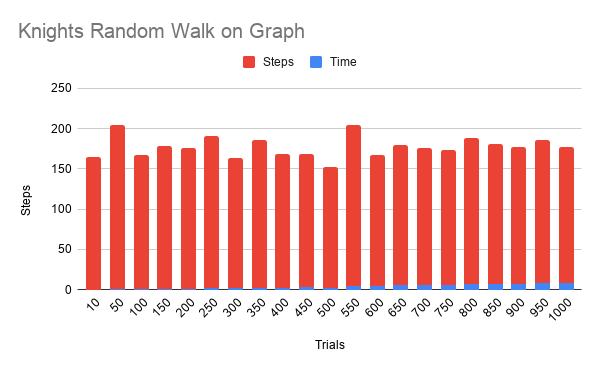
\includegraphics[scale=.60]{image1}
\begin{center}
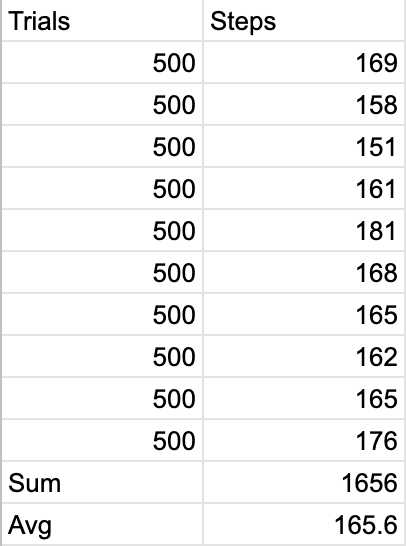
\includegraphics[scale=.60]{image2}
\end{center}

\end{document}
